% !TEX program = xelatex
\documentclass{article}

%% ---- Set up paper margin ---- %%
%\usepackage[a4paper,top=1in,bottom=1in,left=1in,right=1in]{geometry}

% use multiple languages
%% ---- allow CJK usage ---- %%
\usepackage[CJKspace]{xeCJK} % this should be called before Polyglossia
\setCJKmainfont{Noto Serif CJK TC}
\setCJKsansfont{Noto Sans CJK TC}
\setCJKmonofont{Noto Sans Mono CJK TC}
% \setCJKmainfont{Noto Serif JP}
% \setCJKsansfont{Noto Sans JP}
% \setCJKmonofont{Noto Sans Mono CJK JP}

%% ---- ตั้งค่าให้ตัดคำภาษาไทย ---- %%
\XeTeXlinebreaklocale "th"
\XeTeXlinebreakskip = 0pt plus 0pt % เพิ่มความกว้างเว้นวรรคให้ความยาวแต่ละบรรทัดเท่ากัน

%% ---- font settings ---- %%
\usepackage{fontspec}
\defaultfontfeatures{Mapping=tex-text} % map LaTeX formating, e.g., ``'', to match the current font
% To change the main font, uncomment one of the below command.
% \setmainfont{TeX Gyre Termes} % Free Times
% \setsansfont{TeX Gyre Heros} % Free Helvetica
% \setmonofont{TeX Gyre Cursor} % Free Courier
\newfontfamily{\thaifont}[Scale=MatchUppercase,Mapping=textext]{Laksaman} % ตั้งฟอนต์หลักภาษาไทย
\newenvironment{thailang}{\thaifont}{} % create environment for Thai language
\usepackage[Latin,Thai]{ucharclasses} % ตั้งค่าให้ใช้ "thailang" environment เฉพาะ string ที่เป็น Unicode ภาษาไทย
\setTransitionTo{Thai}{\begin{thailang}}
\setTransitionFrom{Thai}{\end{thailang}}

%% ---- spacing between lines ---- %%
\usepackage{setspace}
% \singlespacing % default setting
% \onehalfspacing % recommend using this for Thai language

%% ---- using alphabatic language ---- %%
\usepackage{polyglossia}
\setdefaultlanguage{english} % it is preferrable to set English as the main language, since the numeric system is compatible with most LaTeX features such as 'enumerate' and so on
\setotherlanguages{thai}

\AtBeginDocument\captionsthai % allow captions to be in Thai


%% ---- math packages ---- %%
\usepackage{amsmath}
\usepackage{amssymb}
\usepackage{bm} % same functionality as \mathbf{} but for greek letters
\usepackage{diffcoeff}
\usepackage{physics}
\usepackage{mathdots}
% \numberwithin{equation}{section} % equation numbers are formatted as <#Section>.<#eq in the section>

%% ---- define math environment ---- %%
\usepackage{amsthm}
% \newtheorem{definition}{Definition}[section]
\newtheorem{definition}{Definition}
\newtheorem{proposition}[definition]{Proposition}
\newtheorem{theorem}[definition]{Theorem}
\newtheorem{corollary}{Corollary}[definition]
\newtheorem{remark}{Remark}[definition]
\newtheorem{lemma}[definition]{Lemma}
\newtheorem{problem}[definition]{Problem}
% \newtheorem*{problem}{Problem}

%% ---- hyperref settings ---- %%
\usepackage{hyperref}
\usepackage{url}
\usepackage{cite}
\usepackage{xcolor}
\hypersetup{
    colorlinks,
    linkcolor={red!50!black},
    citecolor={green!50!black},
    urlcolor={blue!80!black}
    }

%% ---- misc. packages ---- %%
\usepackage{enumitem} % allow customizing list environments: enumerate, itemize and description.
\usepackage{mhchem} % use chemistry notation
\usepackage{lipsum}
\usepackage{metalogo} % for extended LaTeX logo such as XeTeX
\usepackage{subcaption} % allowing subfigure environment
% \usepackage[section]{placeins} % ensure floats do not go into the next section and allow the use of \FloatBarrier
\usepackage{graphicx} % allow cropping and rotating images
\usepackage{caption}
\usepackage{float} % allow the use of [H] for positioning of tables and figures
\usepackage{tikz-cd}
\restylefloat{table}

%% ---- title, authors, and dates ---- %%
\usepackage{authblk}
\title{A simple time-dependent model of kidney}
\author[1]{Chanoknun Sintavanuruk}
% \affil[1]{Department of Physiology, Faculty of Medicine Siriraj Hospital, Mahidol University}
% \author[2,3]{XXXX XXXX}
% \affil[2]{Department of XXXX, XXXX University}
% \affil[3]{Department of XXXX, XXXX University}
\date{\today}

\begin{document}
\sloppy % ช่วยตัดคำภาษาไทย
\maketitle

\section{Model equations}

In this model, we consider the medulla of the kidney as a multiphasic continuum consisting of luminal compartments of nephrons and a single combined interstitium-vessel compartment, which we will refer to as simply the interstitium. 
We assume that there is no variation across the medullary tissue of the same depth so that the model can be represented in a one-dimensional spatial domain $(0,L)$, where $x=0$ is the most superficial part of the outer medulla.
Further, we suppose that the population of nephrons is homogeneous, so that we have three distinct luminal compartments: the descending tubules, the ascending tubules, and the collecting tubules.

For each compartment, the occupied volume is given by the volume density (per unit depth) $\alpha_k$, as a function of space and time, where we use $k$ to identify the compartment; $k=0,\mathrm{D},\mathrm{A},\mathrm{C}$ are for the interstitium, the descending, ascending, and collecting tubules respectively.
By assuming the total volume of the medulla is constant, we have
\begin{equation}\label{eq:vol_conserv}
    \sum_k \alpha_k = \alpha_*
\end{equation}
    where $\alpha_*:(0,L)\to \mathbb{R}_+$ is the total volume density of the medulla.

The dynamics of $\alpha_k$ are given by
\begin{align}\label{eq:volume_dynamics}
    \frac{\partial \alpha_k}{\partial t} + \frac{\partial}{\partial x}\left( \alpha_k u_k \right) &= -\gamma_kw_k,\quad k=\mathrm{D},\mathrm{A},\mathrm{C},\\
    \frac{\partial \alpha_0}{\partial t} + \frac{\partial }{\partial x}\left( \alpha_0 u_0 \right) &= \sum_{k=\mathrm{D},\mathrm{A},\mathrm{C}} \gamma_kw_k.
\end{align}
Here, $u_k$ is the water flow velocity, $w_k$ is the transmural flux of the water reabsorbed into the interstitium, and $\gamma_k$ describes the area of the luminal wall per unit depth.
For each compartment $k$, the flow velocity $u_k$ depends on the hydrostatic pressure $p_k$, and is described by the Poiseuille equation:
\begin{equation}
    \frac{\rho_k u_k}{\alpha_k} = -\frac{\partial p_k}{\partial x},\quad k=0,\mathrm{D},\mathrm{A},\mathrm{C},
\end{equation}
    with $\rho_k$ is a constant so that $\rho_k/\alpha_k$ represents the hydraulic resistivity which depends on the volume density $\alpha_k$.
The transmural fluxes $w_k$ on the right-hand side of (\ref{eq:volume_dynamics}) depend on the difference of both the hydrostatic pressures $p_k$ and the osmotic pressures $\pi_k$ between the luminal and the interstitial compartments.
That is,
\begin{equation}
    w_k := \zeta_\mathrm{w}^k\left( \psi_k - \psi_0 \right),\quad \psi_k:=p_k - \pi_k,\quad k=\mathrm{D},\mathrm{A},\mathrm{C}
\end{equation}
    where $\zeta_\mathrm{w}^k$ are the water permeability of the tubules, and $\psi_k$ are called the `water potential'.

We describe the hydrostatic pressure $p_k$ by considering a mechanical property of the nephrons.
We assume that this can be captured by the compliance $\nu_k$, $k=\mathrm{D},\mathrm{A},\mathrm{C}$, of the tubular walls, and we have
\begin{equation}
    \nu_k(p_k - p_0) = \frac{\alpha_k}{\bar{\alpha}_k} - 1,\quad k=\mathrm{D},\mathrm{A},\mathrm{C},
\end{equation}
where $\bar{\alpha}_k$ are the resting volume density for which $p_k = p_0$.
Note that the interstitial hydrostatic pressure is determined by the volume conservation given by (\ref{eq:vol_conserv}).

The osmotic pressure $\pi_k$, on the other hand, depends on the total concentration of the solutes.
In this model, for each compartment $k$, we will only consider two unknown concentrations of solute species: the salt concentration $c_\mathrm{s}^k$, and the urea concentration $c_\mathrm{u}^k$.
The rest of the solute species will be treated as a fixed immobile solute, and we denote the total amount (per unit depth) by $a_k$.
We define the osmotic pressure by
\begin{equation}
    \pi_k:= \sum_{i=\mathrm{s},\mathrm{u}}c_i^k+\frac{a_k}{\alpha_k},\quad k=0,\mathrm{D},\mathrm{A},\mathrm{C}.
\end{equation}

Now, similarly to the dynamics of the volume density, we have equations for the salt and urea concentrations:
\begin{align}\label{eq:solute_dynamics}
    \frac{\partial}{\partial t}\left( \alpha_k c_i^k \right)&=-\frac{\partial}{\partial x} f_i^k - \gamma_kg_i^k,\quad k=\mathrm{D},\mathrm{A},\mathrm{C},\\
    \frac{\partial}{\partial t}\left( \alpha_0 c_i^0 \right)&=-\frac{\partial}{\partial x} f_i^0 + \sum_{k=\mathrm{D},\mathrm{A},\mathrm{C}} \gamma_k g_i^k,
\end{align}
    where $i=\mathrm{s},\mathrm{u}$.
The axial flow and transmural flux of the solute $i$ are denoted by $f_i^k$ and $g_i^k$ respectively.
The axial flow has two components: diffusion and advection.
We write $f_i^k$ as
\begin{equation}
    f_i^k := -{\color{red}\alpha_k}D_i^k\frac{\partial c_i^k}{\partial x}+\alpha_ku_kc_i^k,\quad k=0,\mathrm{D},\mathrm{A},\mathrm{C},
\end{equation}
    where $D_i^k$ are the diffusion coefficients.
{\color{red}Correction: since $f_i^k$ is a \textit{flow} and $-D_i^k\partial c_i^k/\partial x$ is a diffusive \textit{flux}, we should have an additional $\alpha_k$ as indicated above.}
For the transmural fluxes $g_i^k$, we have
\begin{equation}
    g_i^k := j_i^k+h_i^k,\quad k=\mathrm{D},\mathrm{A},\mathrm{C}
\end{equation}
    where $j_i^k$ is the passive transport of the solutes, and $h_i^k$ is the active transport.
We assume that the passive transports take the form:
\begin{equation}
    j_i^k = \zeta_i^k\left( \mu_i^k - \mu_i^0 \right),\quad k=\mathrm{D},\mathrm{A},\mathrm{C},
\end{equation}
    where $\zeta_i^k$ are the permeability of the solute $i$ through the tubules, and $\mu_i^k$ is the chemical potential of the solute $i$ in the compartment $k$:
\begin{equation}
    \mu_i^k:= RT\ln c_i^k,\quad k=0,\mathrm{D},\mathrm{A},\mathrm{C}.
\end{equation}
Note that, since we are considering only salt and urea, we essentially eliminate the need to address the electrical potential, i.e., the electroneutrality condition requires that the movement of \ce{Na+} ions must be accompanied by that of \ce{Cl-} ions, so we can think of salt as having no charge.
The active transport $h_i^k$ represent the transport which requires external energy.
In this case, we are interested the molecular pump of salt from the ascending tubules into the interstitium.
So, $h_\mathrm{s}^\mathrm{A}$ is a non-negative function and $h_i^k\equiv 0$ for $k=\mathrm{D},\mathrm{C}$ or $i=\mathrm{u}$.

Now, we need to specify the boundary conditions.
For the interstitial compartment, we assume no-flux boundary at $x=L$, i.e.,
\begin{align}
    u_0(t,L) &= 0,\\ 
    f_i^0(t,L)&=0,\quad i=\mathrm{s},\mathrm{u}.
\end{align}
On the other hand, we allow interstitial water flow and advective solute flow at $x=0$ in the negative direction.
More precisely,
\begin{align}
    (\alpha_0u_0)(t,0) &= \min\left\{ 0,\frac{P_{\mathrm{v}}-p_0(t,0) }{R_{\mathrm{v}}}\right\},\\ 
    f_i^0(t,0) &= (\alpha_0 u_0 c_i^0)(t,0),\quad i=\mathrm{s},\mathrm{u},
\end{align}
    where $P_{\mathrm{v}}$ is the pressure inside larger vessels which are coupled to the interstitial compartment, and $R_\mathrm{v}$ is the resistance of the coupling.
The rectification is so that we avoid having to specify the solute input from the outside when the pressure $p_0(t,0)$ is less than that of the pressure $P_\mathrm{vessel}$ of larger vessels.
With this same reason, we do not allow diffusive solute flow through this coupling.

For the luminal compartments, we have solute and water input from the proximal tubules in the descending compartment at $x=0$.
Formally, we write
\begin{align}
    (\alpha_\mathrm{D} u_\mathrm{D})(t,0) &= \mathrm{GFR}(t),\\
    f_i^\mathrm{D}(t,0) &= (\alpha_\mathrm{D}u_\mathrm{D}c_i^\mathrm{D})(t,0),\quad i=\mathrm{s,u}\\
    c_i^\mathrm{D}(t,0) &= c_{i}^{\mathrm{filtrate}}(t)
\end{align}
    where $\mathrm{GFR}$ is a non-negative function of time, which can be given or depend on other model unknowns such as the pressure of the descending tubule or the salt concentration in the ascending tubule.
We also have the concentration at the beginning of the descending tubule $c_i^\mathrm{filtrate}$ given.
Furthermore, we have couplings between the descending and ascending tubules at $x=L$ and between the ascending and collecting tubules at $x=0$, i.e., we have
\begin{align}
    (\alpha_\mathrm{D}u_\mathrm{D}+\alpha_\mathrm{A}u_\mathrm{A})(t,L) &= 0,\\
    \quad\left( f_i^\mathrm{D}+f_i^\mathrm{A} \right)(t,L) &= 0,\\
    p_\mathrm{D}(t,L)&= p_{\mathrm{A}}(t,L),\\ 
    c_i^\mathrm{D}(t,L) &=c_i^\mathrm{A}(t,L)
\end{align}
and, similarly,
\begin{align}
    (\alpha_\mathrm{A}u_\mathrm{A}+\alpha_\mathrm{C}u_\mathrm{C})(t,0) &= 0,\\
    \quad\left( f_i^\mathrm{A}+f_i^\mathrm{C} \right)(t,0) &= 0,\\
    p_\mathrm{A}(t,0)&= p_{\mathrm{C}}(t,0),\\ 
    c_i^\mathrm{A}(t,0) &=c_i^\mathrm{C}(t,0),
\end{align}
    where $i = \mathrm{s},\mathrm{u}$.
Note that in our simplification, we are bypassing the distal convoluted tubules in the coupling between the ascending and the collecting tubules.
Finally, since the volume density of the collecting tubule is the model unknown, we need to specify the solute and water flow at $x=L$ where we use the same idea as those of the interstitium:
\begin{align}
    (\alpha_\mathrm{C} u_\mathrm{C} )(t,L) &= \max\left\{ 0,\frac{p_\mathrm{C} (t,L) - P_{\mathrm{p}} }{R_{\mathrm{p}}}\right\},\\
    f_i^\mathrm{C}(t,L) &= (\alpha_\mathrm{C}  u_\mathrm{C}  c_i^\mathrm{C})(t,L),\quad i=\mathrm{s},\mathrm{u},
\end{align}
    where $P_\mathrm{p}$ is the papillary pressure and $R_\mathrm{p}$ is the resistance of the coupling between the collecting tubules and the renal papillae.

\section{Non-dimensionalization}

We now consider the rescaling of space and time:
\begin{equation}
    x = L\hat{x},\quad t = \frac{L^2}{D_*}\hat{t},
\end{equation}
    where $D_*$ is the typical magnitude of the diffusion coefficients across all solutes and compartments.
With this, we rescale the model unknowns as follows:
\begin{gather}
    \alpha_k = \bar{\alpha}\hat{\alpha},\quad c_i^k = c_*\hat{c}_i^k,\quad p_k = p_*\hat{p}_k,
    % \quad u_k = \frac{\bar{\alpha}p_*}{\rho_* L}\hat{u}
\end{gather}
    % where $\bar{\alpha} = \frac{1}{L}\int_0^L\alpha_*(x)\,dx$, and $c_*,p_*,\rho_*$ are the typical magnitudes of all solute concentrations, hydrostatic pressures, and hydraulic resistivity.
    for $k=0,\mathrm{D},\mathrm{A},\mathrm{C}$, where $\bar{\alpha} = \frac{1}{L}\int_0^L\alpha_*(x)\,dx$, and $c_*,p_*$ are the typical magnitudes of solute concentrations and hydrostatic pressures.
Here, the dimensionless unknowns with $\hat{\cdot}$ notation are functions in the rescaled space and time $(\hat{t},\hat{x})$.

We have the model equations in the dimensionless form:
\begin{align}
    \frac{\partial \hat{\alpha}_k}{\partial \hat{t}}  + \mathrm{Pe}\frac{\partial}{\partial \hat{x}}\left( \hat{\alpha}_k \hat{u}_k \right) &= - \hat{w}_k,\\ \label{eq:nd_1steq}
    \frac{\partial\hat{\alpha}_0}{\partial \hat{t}}+\mathrm{Pe}\frac{\partial}{\partial \hat{x}}\left( \hat{\alpha}_0 \hat{u}_0 \right) &=\sum_k \hat{w}_k,\\
    \hat{\nu}_k\left( \hat{p}_k - \hat{p}_0 \right) &= \frac{\hat{\alpha}_k}{\hat{\bar{\alpha}}_k}-1,\\
    \hat{\alpha}_0 + \sum_{k} \hat{\alpha}_k &= \hat{\alpha}_*,\\
    \frac{\partial}{\partial \hat{t}}\left( \hat{\alpha}_k \hat{c}_i^k \right)&=-\frac{\partial}{\partial \hat{x}} \hat{f}_i^k - \hat{g}_i^k,\\
    \frac{\partial}{\partial \hat{t}}\left( \hat{\alpha}_0 \hat{c}_i^0 \right)&=-\frac{\partial}{\partial \hat{x}} \hat{f}_i^0 + \sum_k \hat{g}_i^k,
\end{align}
    for $k=\mathrm{D},\mathrm{A},\mathrm{C}$ and $i=\mathrm{s},\mathrm{u}$, where
\begin{align}
    \hat{u}_\cdot &:= -\frac{\hat{\alpha}_\cdot}{\hat{\rho}_\cdot}\frac{\partial \hat{p}_\cdot}{\partial \hat{x}},\\
    \hat{f}_i^\cdot &:= -{\color{red}\hat{\alpha}_\cdot}\hat{D}_\cdot \frac{\partial \hat{c}_i^\cdot}{\partial \hat{x}} + \mathrm{Pe}(\hat{\alpha}_\cdot\hat{u}_\cdot\hat{c}_i^\cdot),\\
    \hat{w}_k&:= \hat{\zeta}_\mathrm{w}^k\left( \hat{\psi}_k-\hat{\psi}_0 \right),\quad\hat{\psi}_\cdot := \hat{p}_\cdot - \hat{\pi}_.,\quad \hat{\pi}_\cdot := \frac{\hat{a}_\cdot}{\hat{\alpha}_\cdot}+\sum_i \hat{c}_i^\cdot,\\
    \hat{g}_i^k &:= \hat{j}_i^k+\hat{h}_i^k,\quad \hat{j}_i^k :=\hat{\zeta}_i^k(\hat{\mu}_i^k-\hat{\mu}_i^0),\quad \hat{\mu}_i^\cdot:=\ln \hat{c}_i^\cdot\label{eq:nd_lasteq}
\end{align}
    for $k=\mathrm{D},\mathrm{A},\mathrm{C}$ and $i=\mathrm{s},\mathrm{u}$.
The label $\cdot$ here is for $0,\mathrm{D},\mathrm{A},\mathrm{C}$.
{\color{red}Correction: as in the previous section, the diffusive term should have an additional $\hat{\alpha}_\cdot$}.
Note that we have $h_i^k = \gamma_k\hat{h}_i^k$ for the dimensionless active transport $\hat{h}_i^k$.
In this dimensionless formulation, we have identified parameters:
\begin{gather}
    \mathrm{Pe} = \frac{\bar{\alpha}p_*/\rho_*}{D_*},\quad \hat{\rho}_\cdot = \frac{\rho_\cdot}{\rho_*},\quad \hat{\nu}_k = p_*\nu_k,\quad \hat{\bar{\alpha}}_\cdot = \frac{\bar{\alpha}_\cdot}{\bar{\alpha}},\quad \hat{\alpha}_* = \frac{\alpha_*}{\bar{\alpha}}\\
    \hat{a}_\cdot = \frac{a_\cdot}{\bar{\alpha}c_*},\quad
    \hat{D}_\cdot = \frac{D_\cdot}{D_*},\quad \hat{\zeta}_\mathrm{w}^k = \frac{\gamma_k c_*L^2}{\bar{\alpha}D_*}\zeta_\mathrm{w}^k,\quad\hat{\zeta}_i^k = \frac{\gamma_kRT L^2}{\bar{\alpha}c_* D_*}\zeta_i^k,
\end{gather}
    for $k=\mathrm{D},\mathrm{A},\mathrm{C}$, where the subscript $*$ denotes the typical magnitudes of the parameters described in the previous section.
We have the P\'eclet number $\mathrm{Pe}$ which can be interpreted as the ratio between the rate of advection $\bar{\alpha}p_*/\rho_*L$ and the rate of diffusion $D_*/L$.
The mechanical parameters, which are the hydraulic resistivity $\hat{\rho}_\cdot$, the tubular compliance $\hat{\nu}_\cdot$, and the resting volume density $\hat{\bar{\alpha}}_\cdot$, together with immobile solutes $\hat{a}_\cdot$ and the diffusion coefficients $\hat{D}_\cdot$, persist through the non-dimensionalization.
The transport parameters, however, are now reduced to only $\hat{\zeta}_\mathrm{w}^k$ and $\hat{\zeta}_i^k$ which combine the geometric parameters $\gamma_k$ with the solute and water permeability.

For the boundary conditions, we have the same form as previously described, but with $\hat{\cdot}$ notations, where we have
\begin{equation}
    \mathrm{GFR} = \frac{\bar{\alpha}^2 p_*}{\rho_* L}\widehat{\mathrm{GFR}},\quad
    P_\cdot = p_*\hat{P}_\cdot,\quad R_\cdot = \frac{\rho_* L}{\bar{\alpha}^2}\hat{R}_\cdot,
\end{equation}
    where the subscript $\cdot$ represents $\mathrm{v}$ and $\mathrm{p}$.

\section{Numerical method}

% \begin{align}
%     \frac{\partial \alpha_k}{\partial t}  + \mathrm{Pe}\frac{\partial}{\partial x}\left( \alpha_k u_k \right) &= - w_k,\\
%     \frac{\partial\alpha_0}{\partial t}+\mathrm{Pe}\frac{\partial}{\partial x}\left( \alpha_0 u_0 \right) &=\sum_k w_k,\\
%     \frac{\partial}{\partial t}\left( \alpha_k c_i^k \right)&=-\frac{\partial}{\partial x} f_i^k - g_i^k,\\
%     \frac{\partial}{\partial t}\left( \alpha_0 c_i^0 \right)&=-\frac{\partial}{\partial x} f_i^0 + \sum_k g_i^k,\\
%     \nu_k\left( p_k - p_0 \right) &= \frac{\alpha_k}{\bar{\alpha}_k}-1,\\
%     \alpha_0 + \sum_{k} \alpha_k &= \alpha_*,
% \end{align}
% \begin{align}
%     \frac{\rho_\cdot}{\alpha_\cdot}u_\cdot &= -\frac{\partial p_\cdot}{\partial x},\\
%     f_i^\cdot&= -D_i^\cdot\frac{\partial c_i^\cdot}{\partial x}+\mathrm{Pe}\left( \alpha_\cdot u_\cdot c_i^\cdot \right),\\
%     % f_i^\cdot&= -D_i^\cdot c_i^\cdot\frac{\partial \mu_i^\cdot}{\partial x}+\mathrm{Pe}\left( \alpha_\cdot u_\cdot c_i^\cdot \right),\quad \mu_i^\cdot:=\ln c_i^k \\
%     w_k&= \zeta_k\left( \psi_k-\psi_0 \right),\quad\psi_\cdot := p_\cdot - \pi_.,\quad \pi_\cdot := \frac{a_\cdot}{\alpha_\cdot}+\sum_i c_i^\cdot,\\
%     g_i^k &= j_i^k+h_i^k,\quad j_i^k :=\gamma_i^k(\mu_i^k-\mu_i^0).
%     % := \ln\left( \frac{c_i^k}{c_i^0} \right).
% \end{align}

We now give an implicit scheme to numerically solve the dimensionless system (\ref{eq:nd_1steq}) - (\ref{eq:nd_lasteq}) described in the previous section.
To simplify the notation, we will omit the $\hat{\cdot}$ notation in these equations.

Let $N\in \mathbb{N}$ be the number of uniformly spaced grids in $(0,1)$, and $\delta x = 1/N$ be the spatial grid size.
Similarly, we denote $\delta t$ as the size of time steps.
We will use the notation $\alpha^{n}_{kl},c_{il}^{kn}, p_{kl}^{n}$ for the discretization of $\alpha_k,c_i^k$ and $p_k$ at the $l$-th spatial grid and time $t = n\delta t$.
These correspond to the values in between the spatial grid point, e.g., $\alpha_{kl}^n$ corresponds to $\alpha_k(n\delta t,l-\delta x/2)$.

We define difference quotient operators:
\begin{equation}
    \mathcal{D}_x^+y^n_l:= \frac{y^n_{l+1}-y^n_{l}}{\delta x},\quad \mathcal{D}_x^- y^n_l :=\frac{y^n_l-y^n_{l-1}}{\delta x},\quad \mathcal{D}_t y^n_l = \frac{y^n_l - y^{n-1}_l}{\delta t},
\end{equation}
and an average operator:
\begin{equation}
    \mathcal{A} y_l^n := \frac{y^n_{l+1}+y^n_l}{2},
\end{equation}
    where $\{y_l^n\}$ is any discretized variables with $l,n\in \mathbb{N}\cup\{0\}$.

Starting with known values of $\alpha^{n-1}_{kl},c_{il}^{k,n-1}, p_{kl}^{n-1}$, $l = 1,\dots,N$, the first step is to update the unknowns for the next time step $n$.
We have the system of equations for $\alpha^{n}_{kl},c_{il}^{kn}, p_{kl}^{n}$, $l=1,\dots,N$, to be solved using an iterative method:
\begin{align}
    \mathcal{D}_t \alpha_{kl}^n +\mathrm{Pe}\mathcal{D}_x^-v_{kl}^n &= \begin{cases}
        -w_{kl}^{n},\quad &k=\mathrm{D},\mathrm{A},\mathrm{C},\\
        \sum_{\kappa\neq 0} w_{\kappa l}^n, &k=0,
    \end{cases}\\
    \mathcal{D}_t (\alpha_{kl}^nc_{il}^{kn})+\mathcal{D}_x^-f_{il}^{kn}&=\begin{cases}
        -g_{k n}^{il}, &k=\mathrm{D},\mathrm{A},\mathrm{C},\\
        \sum_{\kappa \neq 0}g_{il}^{\kappa n}, &k=0.
    \end{cases}\\
    p_{kl}^n &= \begin{cases}
        p_{0l}^n + \frac{1}{\nu_k}\left( \frac{\alpha_{kl}^n}{\bar{\alpha}_{kl}} - 1\right),\quad &k=\mathrm{D},\mathrm{A},\mathrm{C},\\
        \frac{\alpha_{0l}^n - \alpha_* + \sum_{\kappa\neq 0}\bar{\alpha}_\kappa (\nu_\kappa p_\kappa +1)}{\sum_{\kappa\neq 0}\bar{\alpha}_\kappa \nu_\kappa }, &k=0.
    \end{cases}
\end{align}
where the transmural flux terms $w_{kl}^n$ and $g_{il}^{kn}$ are the discritization of $w_k$ and $g_i^k$ on the same grid as the unknowns:
\begin{align}
    w_{kl}^n &:=\zeta_\mathrm{w}^k\left( \psi_{kl}^n-\psi_{0l}^n \right),\quad
    \psi_{\cdot l}^n:= p_{\cdot l}^n - \pi_{\cdot l}^n,\quad \pi_{\cdot l}^n:= \sum_i c_{il}^{\cdot n},\\
    g_{il}^{kn}&:= j_{il}^{kn}+h_{il}^{kn},\quad j_{il}^{kn}:=\zeta_i^k\left( \mu_{il}^{kn} - \mu_{il}^{0n} \right),\quad \mu_{il}^{\cdot n}:= \ln c_{il}^{\cdot}.
\end{align}
Here, the axial flows of water $v_{kl}^n$ and solutes $f_{il}^{kn}$ are assigned for $l=0,\dots,N$.
These should be thought as the flow at the \textit{grid points}, e.g., $f_{il}^{kn}$ corresponds to $f_i^k(n\delta t,l\delta x)$.
For $l=1,\dots,N-1$, we have
\begin{align}
    v_{kl}^n &= -\frac{1}{\rho_{kl}}(\mathcal{A}\alpha_{kl}^n)^2 \mathcal{D}_x^+p_{kl}^n,\\
    f_{il}^{kn} &= -{\color{red}(\mathcal{A}\alpha_{kl}^n)}D_{i}^k \mathcal{D}_x^+ c_{il}^{kn}+ v_{kl}^n \mathcal{A}c_{il}^{kn}.
\end{align}
    % where the parameters $D_{il}^k$ and $\rho_{kl}$ are given for $l=0,\dots,N$.

Further, we have the boundary conditions ($l=0,N$):
\begin{alignat}{2}
    v_{00}^n &= \min\left\{ 0,\frac{P_\mathrm{v}(n\delta t) - p_{01}^n}{R_{\mathrm{v}}} \right\},\quad &&f_{00}^n = v_{00}^n,\\
    v_{0N}^n &= 0,\quad &&f_{0N}^n = 0,\\
    v_{\mathrm{D}0}^n &= \mathrm{GFR}(n\delta t),\quad && f_{i0}^{\mathrm{D}n} = v_{\mathrm{D} 0}^nc_i^\mathrm{filtrate}(n\delta t),\\
    v_{\mathrm{C}N}^n &= \max\left\{ 0,\frac{p_{\mathrm{C}N}^n - P_\mathrm{p}(n\delta t)}{R_\mathrm{p}} \right\},\quad && f_{iN}^{\mathrm{C}n} = v_{\mathrm{C} N}^nc_{iN}^{\mathrm{C}n}.
\end{alignat}
For the coupling between the descending and ascending, we have
\begin{align}
    v_{kN}^n &= \frac{(\alpha_{kN}^n)^2}{\rho_k}\left( \frac{p_{kN}^n - \bar{p}_{\mathrm{DA}}^n}{\delta x/2} \right),\\ 
    f_{iN}^{kn} &= -D_i^k\left( \frac{c_{iN}^{kn} - \bar{c}_{i,\mathrm{DA}}^{n}}{\delta x/2} \right)+\mathrm{Pe}v_{kN}^{n}\bar{c}_{i,\mathrm{DA}}^{n},
\end{align}
    for $k=\mathrm{D},\mathrm{A}$, where
\begin{equation}
    \bar{p}_{\mathrm{DA}}^n:=\frac{\frac{(\alpha_{\mathrm{D}N}^n)^2}{\rho_\mathrm{D}}p_{\mathrm{D}N}^n+\frac{(\alpha_{\mathrm{A}N}^n)^2}{\rho_\mathrm{A}}p_{\mathrm{A}N}^n}{\frac{(\alpha_{\mathrm{D}N}^n)^2}{\rho_\mathrm{D}}+\frac{(\alpha_{\mathrm{A}N}^n)^2}{\rho_\mathrm{A}}},\quad 
    \bar{c}_{i,\mathrm{DA}}^n:=\frac{{\color{red}\alpha_{\mathrm{D}N}^n}D_i^\mathrm{D}c_{iN}^{\mathrm{D}n}+{\color{red}\alpha_{\mathrm{A}N}^n}D_i^\mathrm{A}c_{iN}^{\mathrm{A}n}}{{\color{red}\alpha_{\mathrm{D}N}^n}D_i^\mathrm{D}+{\color{red}\alpha_{\mathrm{A}N}^n}D_i^\mathrm{A}}.
\end{equation}
These are so that we have the coupling satisfies $v_{\mathrm{D} N}^n+v_{\mathrm{A} N}^n = 0$, and $f_{iN}^{\mathrm{D}n}+ f_{iN}^{\mathrm{A}n} = 0$.
Here, $\bar{p}_{\mathrm{DA}}^n$ and $\bar{c}_{i,\mathrm{DA}}^n$ correspond to the pressures and the concentrations at $x=1$ of the descending and the ascending tubules.
Likewise, we also have a similar condition for the coupling between the ascending and the descending tubules:
\begin{align}
    v_{k0}^n &= \frac{(\alpha_{k0}^n)^2}{\rho_k}\left( \frac{\bar{p}_{\mathrm{AC}}^n-p_{k0}^n}{\delta x/2} \right),\\ 
    f_{i0}^{kn} &= -D_i^k\left( \frac{\bar{c}_{i,\mathrm{AC}}^{n}- c_{i0}^{kn}}{\delta x/2} \right)+\mathrm{Pe}v_{k0}^{n}\bar{c}_{i,\mathrm{AC}}^{n},
\end{align}
    for $k=\mathrm{A},\mathrm{C}$, where
\begin{equation}
    \bar{p}_{\mathrm{AC}}^n:=\frac{\frac{(\alpha_{\mathrm{A} 0}^n)^2}{\rho_\mathrm{A} }p_{\mathrm{A} 0}^n+\frac{(\alpha_{\mathrm{C} 0}^n)^2}{\rho_\mathrm{C} }p_{\mathrm{C} 0}^n}{\frac{(\alpha_{\mathrm{A} 0}^n)^2}{\rho_\mathrm{A} }+\frac{(\alpha_{\mathrm{C} 0}^n)^2}{\rho_\mathrm{C} }},\quad 
    \bar{c}_{i,\mathrm{AC}}^n:=\frac{{\color{red}\alpha_{\mathrm{A} 0}^n}D_i^\mathrm{A} c_{i0}^{\mathrm{A} n}+{\color{red}\alpha_{\mathrm{C} 0}^n}D_i^\mathrm{C} c_{i0}^{\mathrm{C} n}}{{\color{red}\alpha_{\mathrm{A} 0}^n}D_i^\mathrm{A} +{\color{red}\alpha_{\mathrm{C} 0}^n}D_i^\mathrm{C} }.
\end{equation}


\section{Simulation of the countercurrent mechanism}

In this simulation, we will use a simple geometry of $\alpha_* \equiv 1$, with mechanical parameters $\bar{\alpha}_k = 1/4$ and $\nu_k = 0.01$ for $k=\mathrm{D},\mathrm{A},\mathrm{C}$.
We suppose that $D_\mathrm{s}^k = D_{\mathrm{u}}^k = 1$, $\mathrm{Pe} = 20$, $\rho_k = 1$ for all $k$, and we assume that there is only immobile solute in the interstitium, where we have $a_0 = 1/2$ and $a_k = 0$ for luminal compartments.
Furthermore, we set the resistance of the coupling with larger vessels and the renal papillae $R_\mathrm{v} = R_\mathrm{p} = 1$.

For the transport parameters, we allow the passive transport of salt only in the descending and the ascending tubules, where we set $\zeta_{\mathrm{s}}^\mathrm{D} = \zeta_{\mathrm{s}}^\mathrm{A} = 1$ and $\zeta_{\mathrm{s}}^\mathrm{C} = 0$.
Additionally, all the tubular segments are permeable to urea in the inner medulla, i.e., $\zeta_{\mathrm{u}}^k = 10$ for all $k$ and $x\in (\frac{1}{2},1)$ and $\zeta_{\mathrm{u}}^k =0$ elsewhere.
Furthermore, for illustrating purpose, we consider a simple active transport of salt in the outer medulla of the form
    \begin{equation}
        h_\mathrm{s}^\mathrm{A} = \begin{cases}
            h_*c_\mathrm{s}^\mathrm{A},\quad  &\text{in}\quad (0,\frac{1}{2}),\\
            0\quad &\text{in}\quad [\frac{1}{2},1),
        \end{cases}
    \end{equation}
    where $h_*>0$ is the pump strength, which we set to be $h_*=50$.
For the water transport, the descending tubule will be highly permeable to water with $\zeta_\mathrm{w}^\mathrm{D} = 100$ while the ascending tubule will be completely insulated with $\zeta_\mathrm{w}^\mathrm{A} = 0$. 
We will consider two cases for the collecting tubules: without ADH, in which we have $\zeta_{\mathrm{w}}^\mathrm{C} = 0$, and when there is some ADH so that $\zeta_{\mathrm{w}}^\mathrm{C} = 50$.

We initialize the simulation by setting the initial condition to be no axial solute and flow with 
\begin{gather}
    \alpha_k(0,x) = \frac{1}{4},\quad
    c_\mathrm{s}^k(0,x) = 1,\quad
    c_{\mathrm{u}}^k(0,x) = \frac{1}{4},\quad
    p_k(0,x) = P_\mathrm{v} = P_{\mathrm{p}} = 1   
\end{gather}
    for all $x\in (0,1)$ and $k=0,\mathrm{D},\mathrm{A},\mathrm{C}$.
Then, the glomerular filtration rate gradually increases until it reaches $2.5$:
\begin{equation}
    \mathrm{GFR}(t) = \min\{2.5, t/8\}.
\end{equation}

\subsection{Results}

\begin{figure}
    \centering
    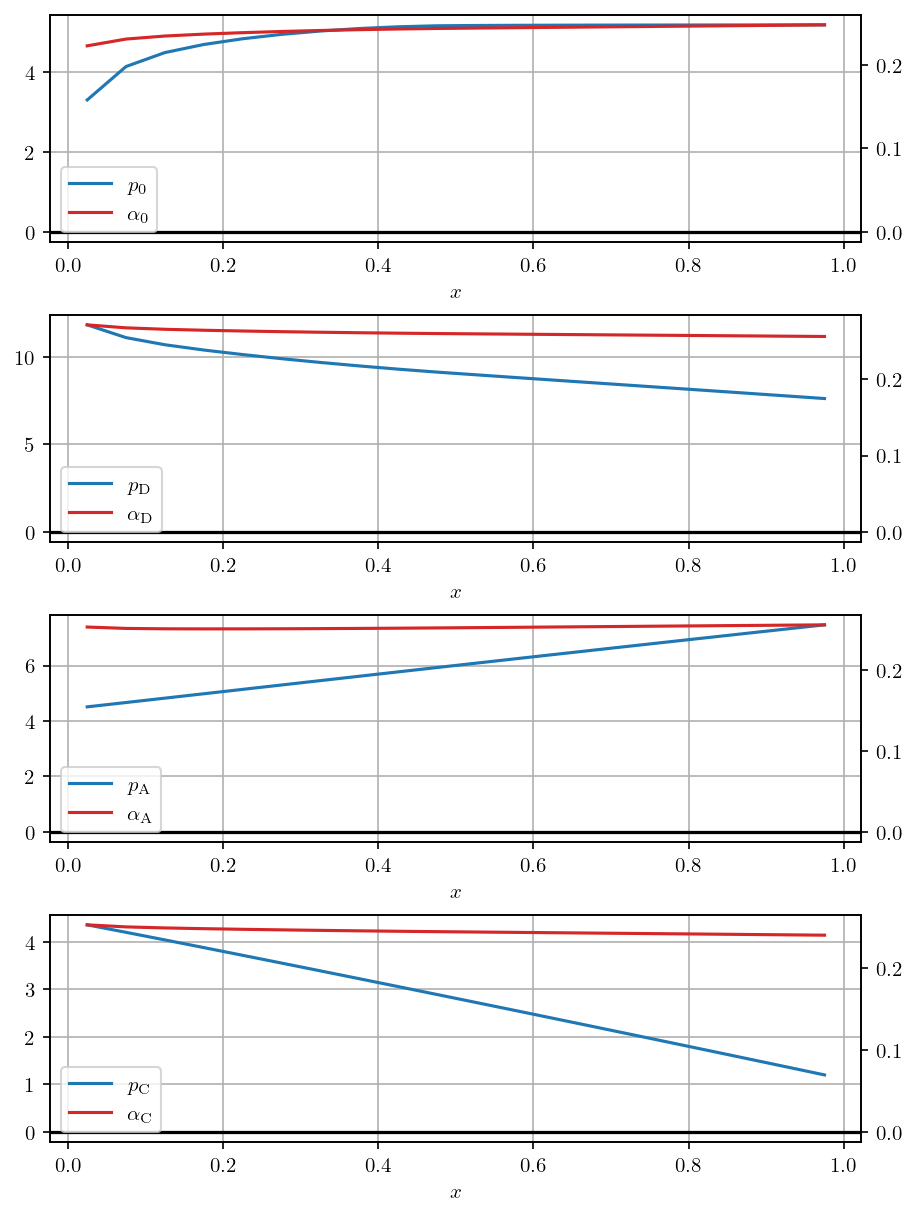
\includegraphics[width=.9\textwidth]{../results/4-7-2023/noADH_p_alpha.png}
    \caption{The pressures and volume densities without ADH}
\end{figure}

\begin{figure}
    \centering
    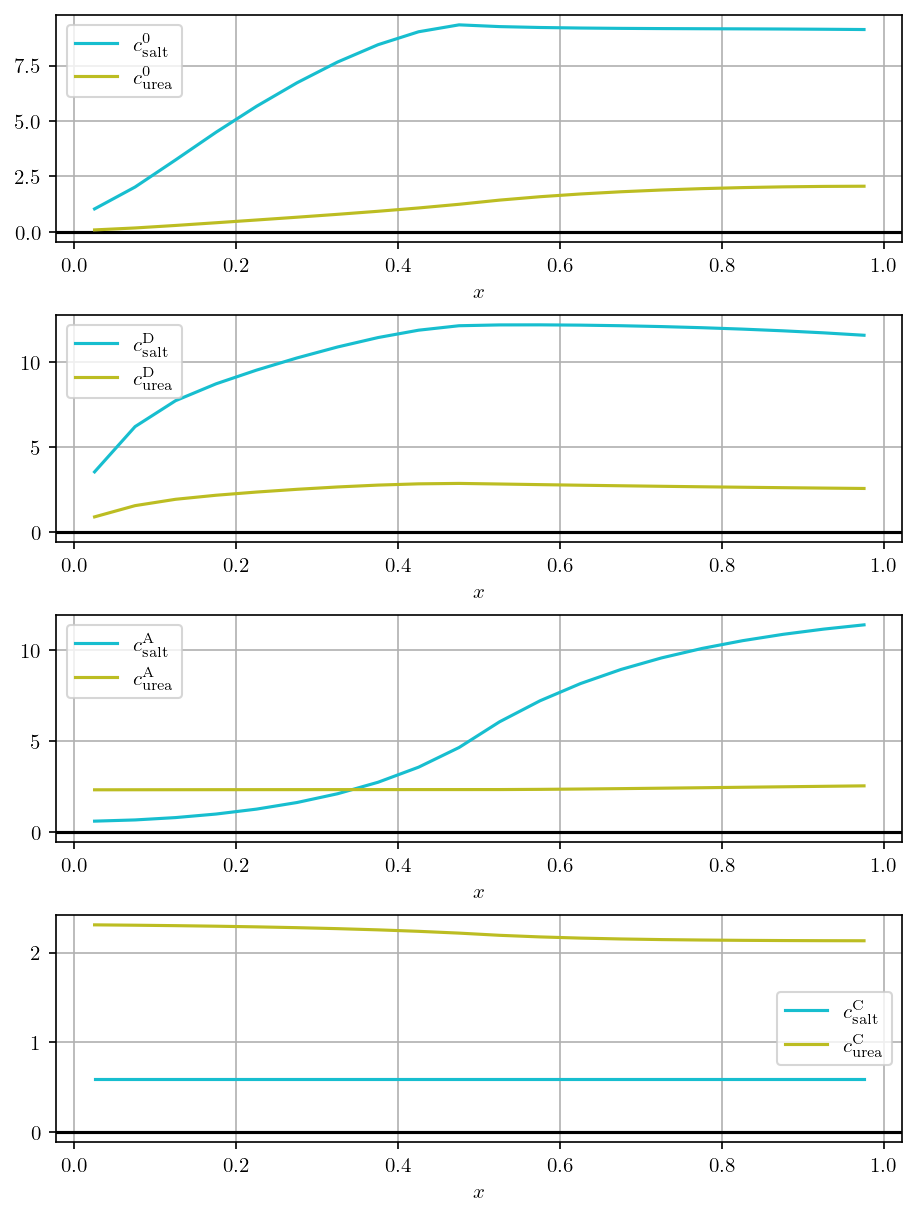
\includegraphics[width=.9\textwidth]{../results/4-7-2023/noADH_c.png}
    \caption{The concentration of salt and urea without ADH}
\end{figure}

\begin{figure}
    \centering
    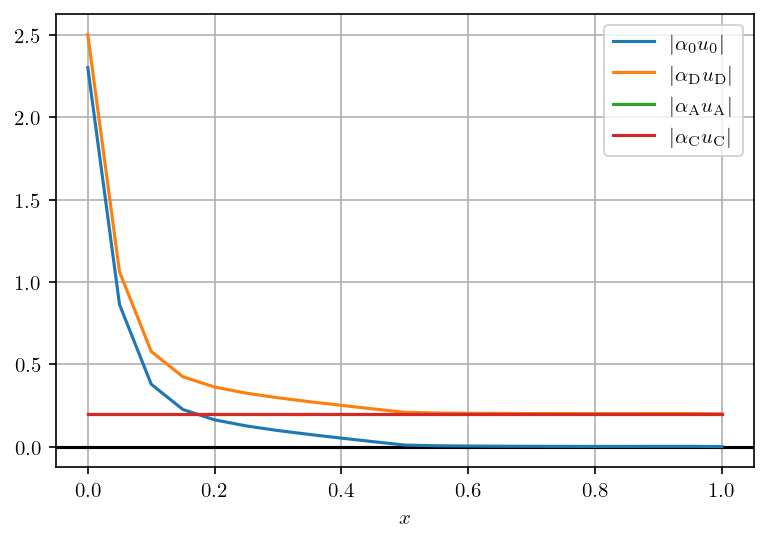
\includegraphics[width=.9\textwidth]{../results/4-7-2023/noADH_flows.png}
    \caption{The water flow without ADH}
\end{figure}

\begin{figure}
    \centering
    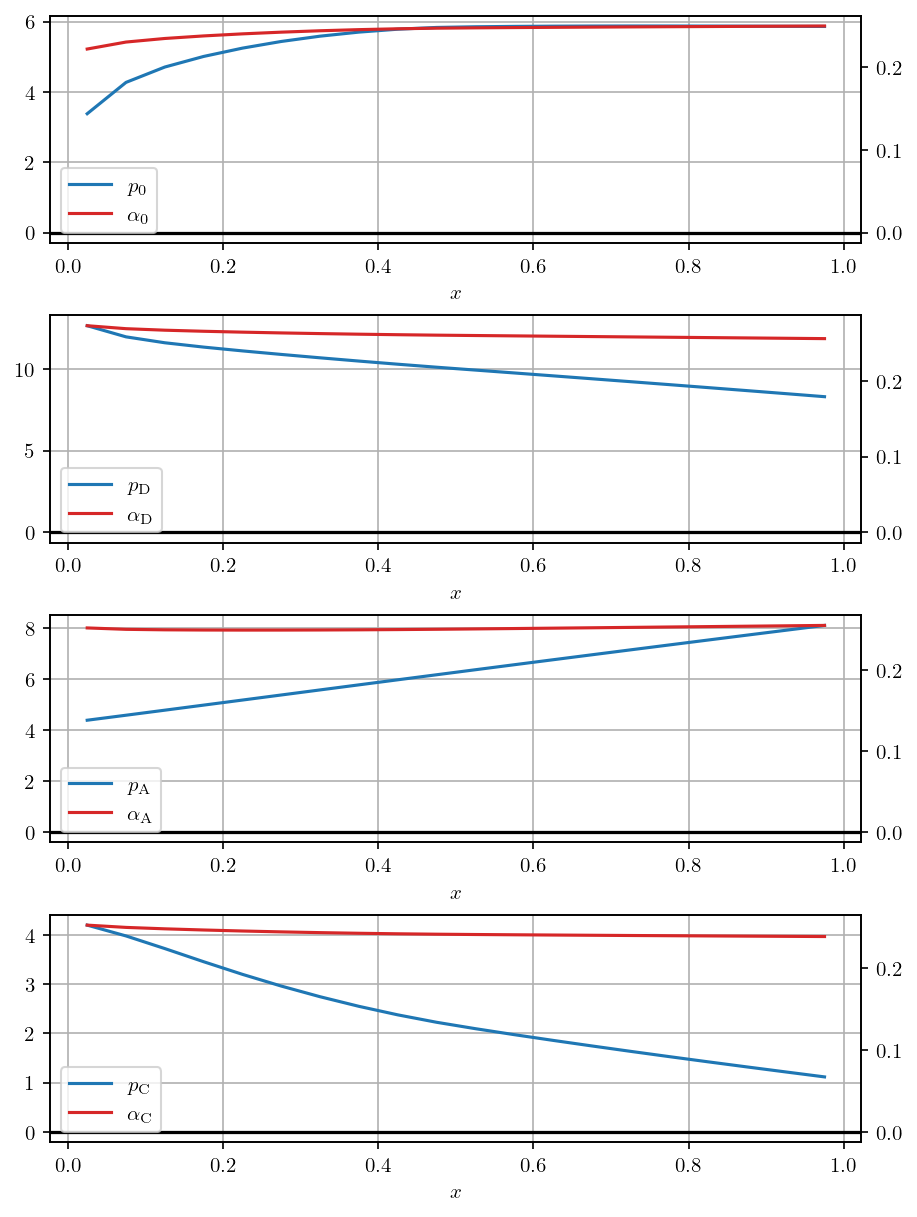
\includegraphics[width=.9\textwidth]{../results/4-7-2023/ADH_p_alpha.png}
    \caption{The pressures and volume densities with ADH}
\end{figure}

\begin{figure}
    \centering
    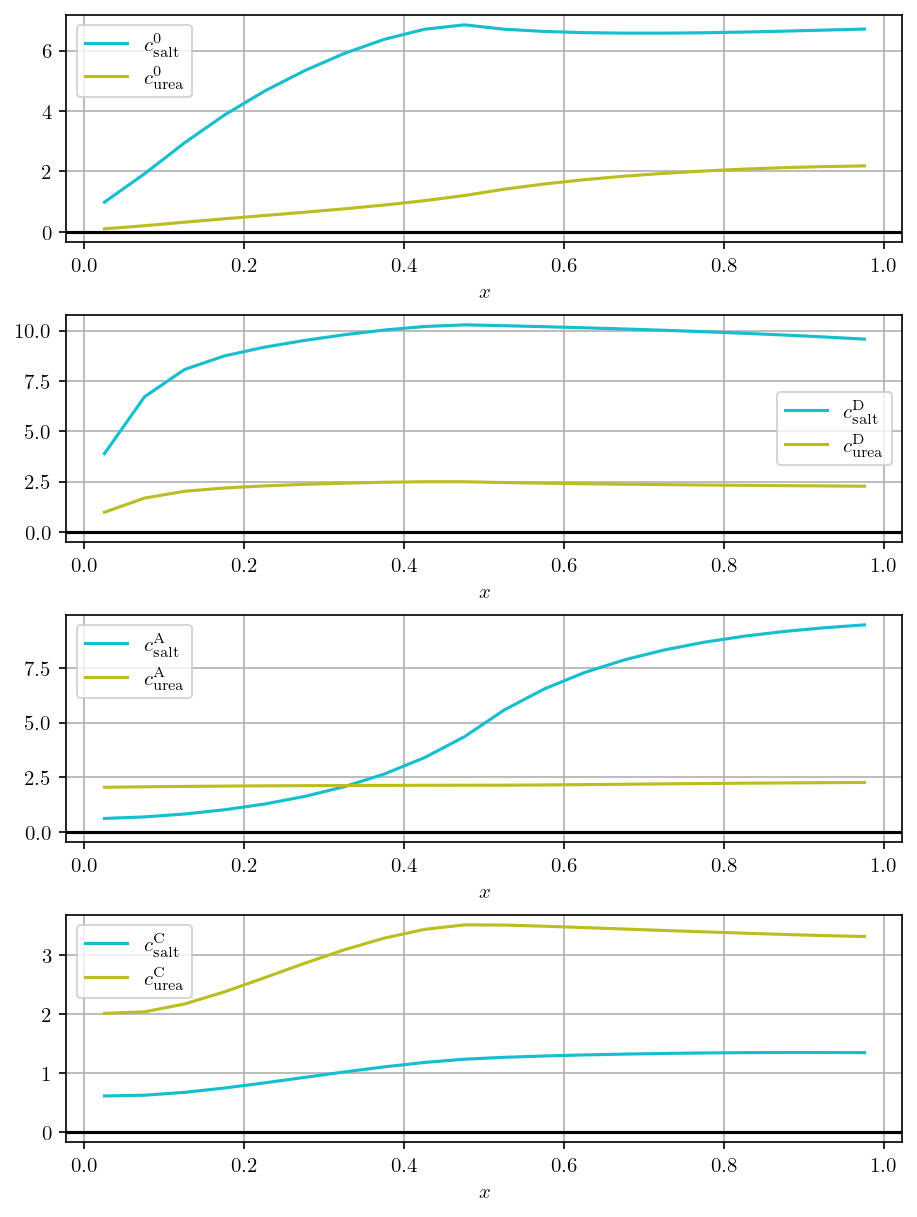
\includegraphics[width=.9\textwidth]{../results/4-7-2023/ADH_c.png}
    \caption{The concentration of salt and urea with ADH}
\end{figure}

\begin{figure}
    \centering
    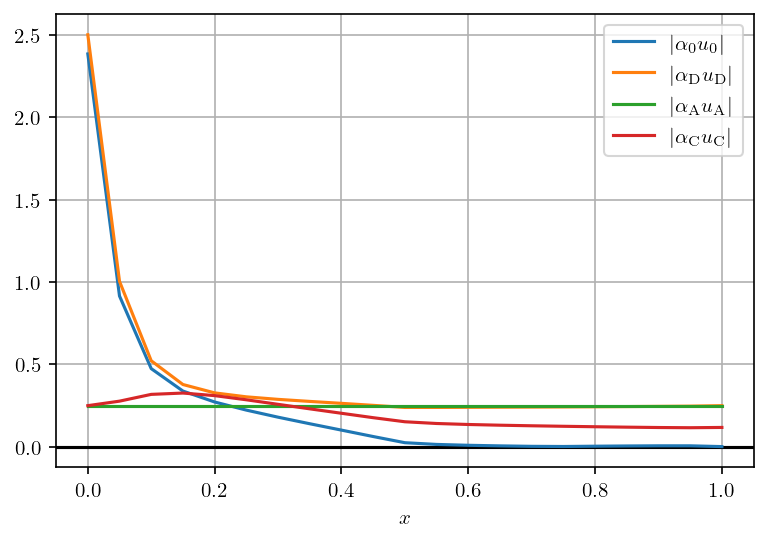
\includegraphics[width=.9\textwidth]{../results/4-7-2023/ADH_flows.png}
    \caption{The water flow with ADH}
\end{figure}


\end{document}